%% The following is a directive for TeXShop to indicate the main file
%%!TEX root = diss.tex

\chapter{Results}
\label{ch:Results}

\section{Fast Simulation Performance}
It was found that the fast ARICH simulation takes approximately 4 seconds to generate a photon distribution resulting from simulating 10,000 particles when running on a computer with a 2.7 GHz processor. 
Simulating the same 10,000 particles on the same computer using the Geant4 simulation of the EMPHATIC setup took approximately 100 seconds.
By ignoring all irrelevant physical processes in the simulation and removing the majority of the overhead of a Geant4 simulation, a significant performance speedup was attained.

\section{Particle Separation}
It is necessary to establish the effectiveness of the likelihood particle identification technique under different conditions.
As an example, let us suppose we want to determine how well this likelihood approach works on a particle that is 7 GeV and measured to enter the center of the aerogel and travel directly in the $z$-direction.
To check the certainty with which this technique can identify whether this is a pion or kaon, I applied the following procedure:

\begin{enumerate}
\item Generate 10,000 pions with the given position, direction, and momenta in Geant4, project the generated Cherenkov photons onto a plane representing the detector, apply efficiency corrections, and store the resulting histogram of detected photon hits for each pion. 
\item Do the same, but with simulated kaons instead of pions.
\item Given the particle initial position, initial direction, and momentum, use the fast ARICH simulation to generate two photon probability distribution histograms, corresponding to pions or kaons.
\item For each event simulated using Geant4, compute the negative log-likelihood of the event histogram with respect to the photon probability distribution functions of each particle hypothesis.
\item For each true particle type, plot a histogram of the log of the ratio of likelihoods between the two hypotheses.
This is just the differences between the negative log-likelihoods of the two hypotheses.
\item Look at the separation between the distributions: this is equal to the difference in means between the distributions, divided by the root mean square of each distribution added in quadrature
\end{enumerate}

The result of this procedure is shown in Figure \ref{fig:kaonpionsep}. The two distributions are separated by a distance of $1.9 \sigma$ - the significant overlap between the two distribution indicates that there is some chance of misidentification. Applying the same procedure to verify the separation between kaons and protons gives the results shown in Figure \ref{fig:kaonprotonsep}. Here we see that the two distributions do not significantly overlap and have a separation of $4.7 \sigma$, meaning that at this momentum and angle, protons are very unlikely to be misidentified as kaons, and vice versa.
\begin{figure}[]
\centering
\resizebox{0.9\textwidth}{!}{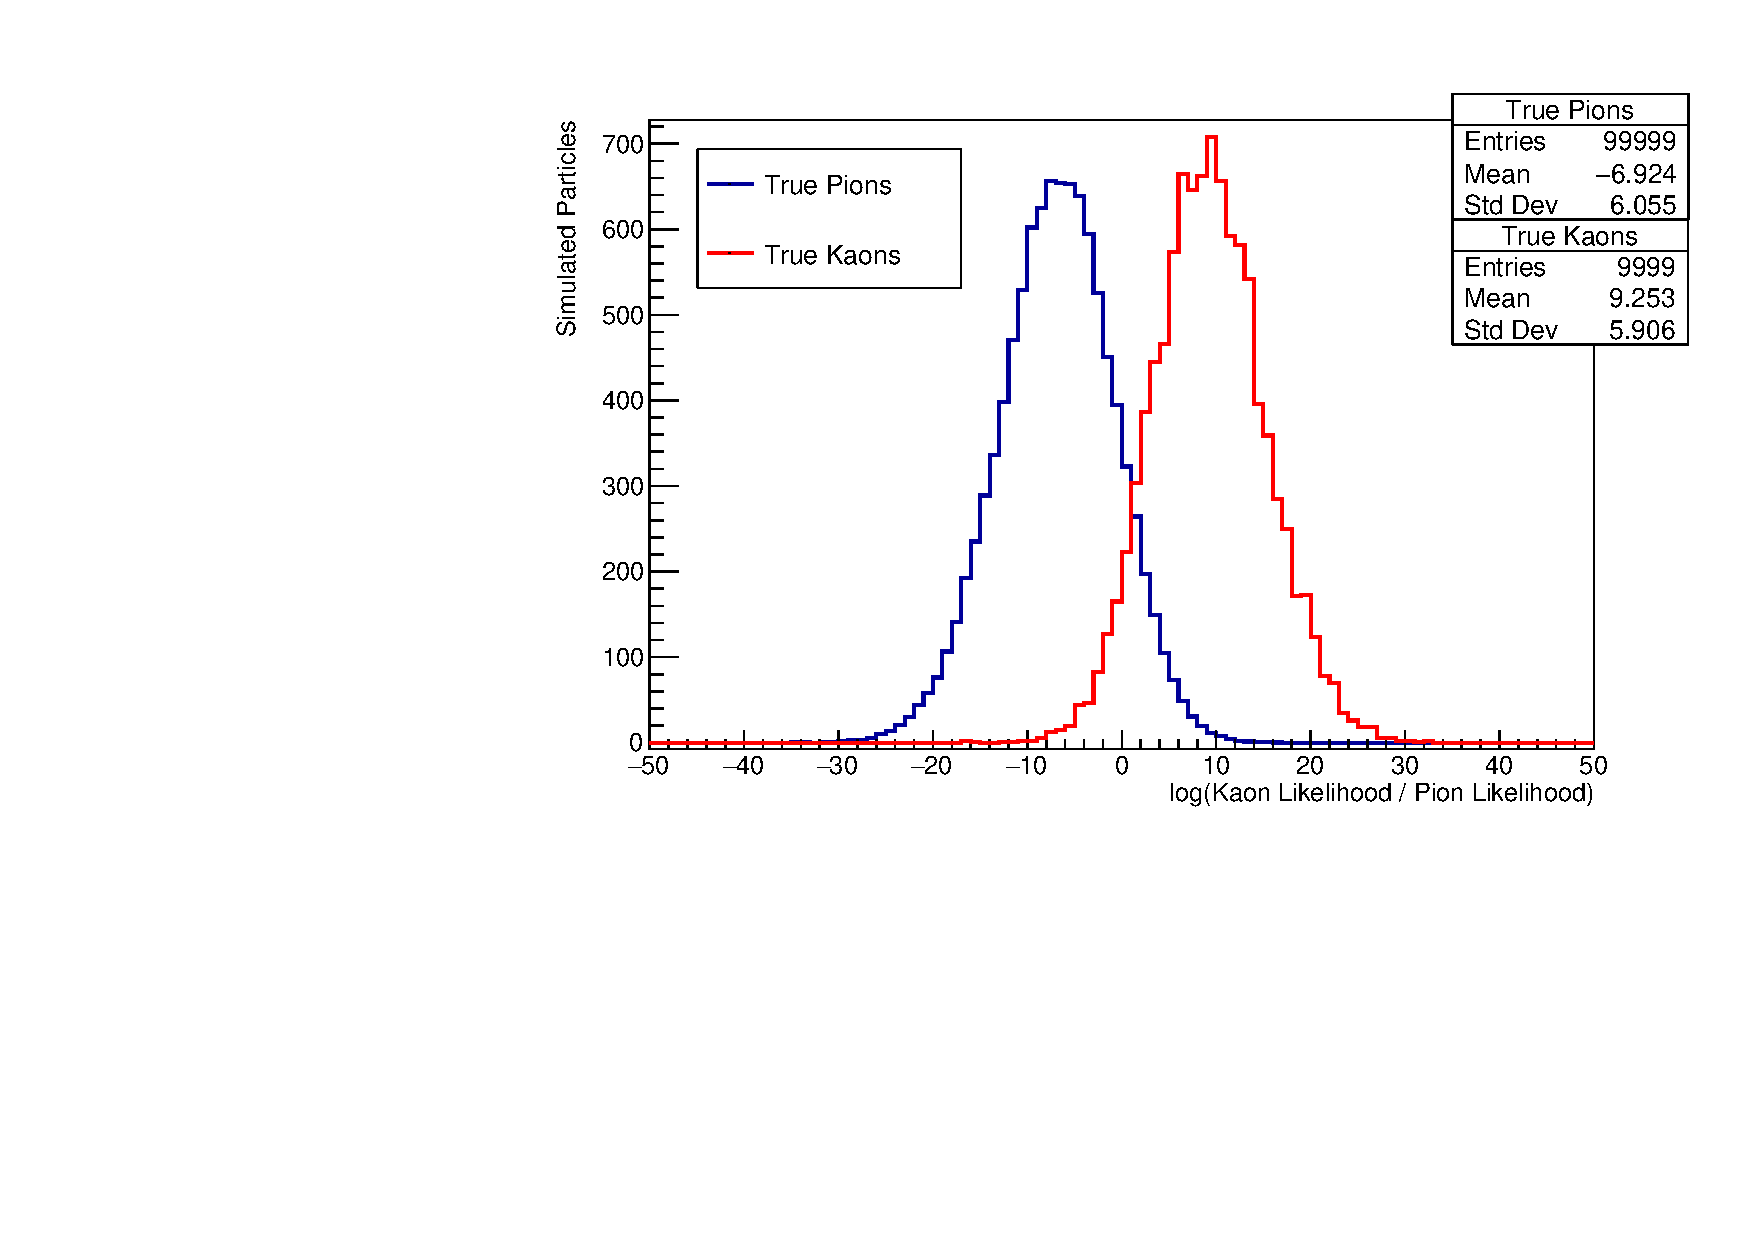
\includegraphics{./figs/kaonPionSep.pdf}}
\caption[Particle identification separation for 7 GeV/c pions and kaons]{Histogram showing the logarithm of the ratios of likelihoods between 7 GeV/c kaons and pions for both ``true" kaons and ``true" pions. The two distributions have a separation of 1.9 $\sigma$.}
\label{fig:kaonpionsep} 
\end{figure}

\begin{figure}[]
\centering
\resizebox{0.9\textwidth}{!}{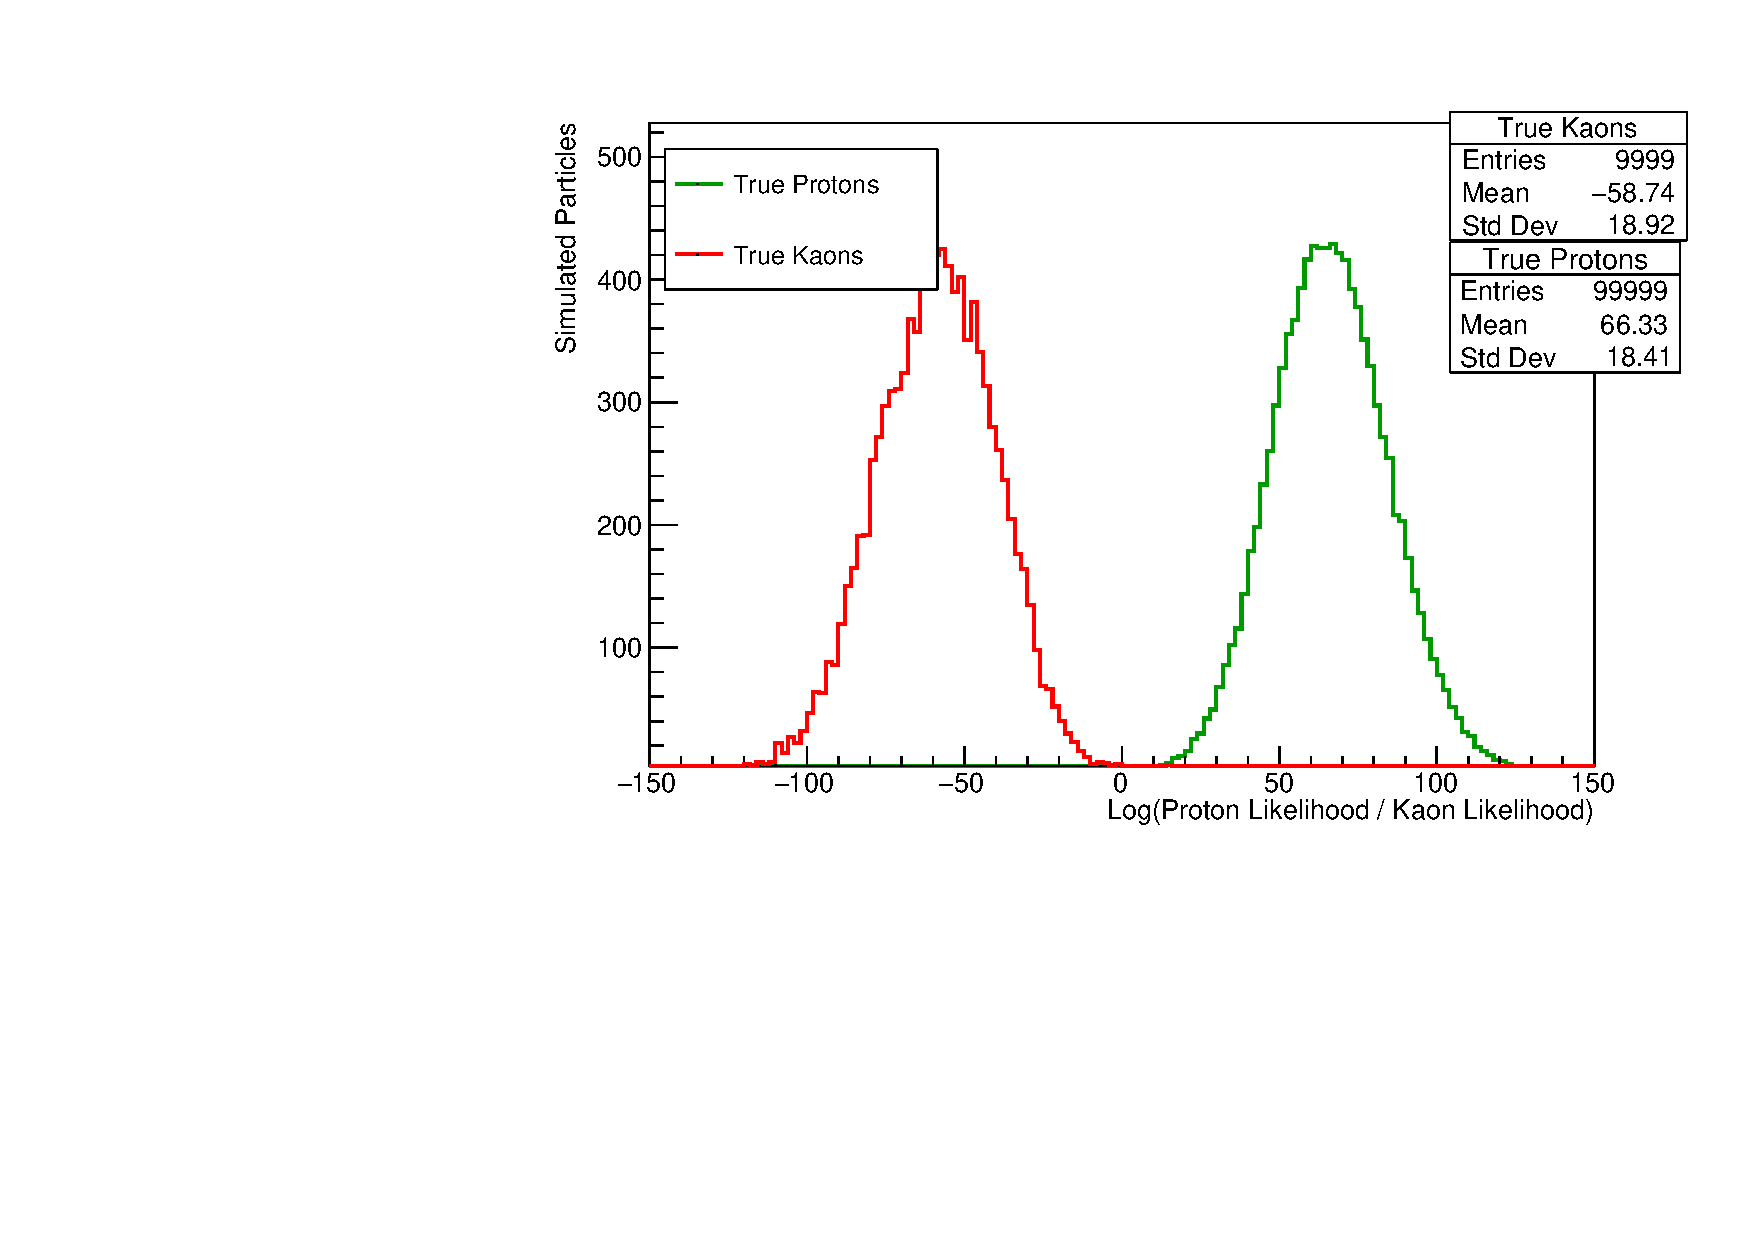
\includegraphics{./figs/kaonProtonSep.pdf}}
\caption[Particle identification separation for 7 GeV/c kaons and protons]{Histogram showing the logarithm of the ratios of likelihoods between 7 GeV/c protons and kaons for both ``true" protons and ``true" kaons. The two distributions have a separation of  4.7 $\sigma$.}
\label{fig:kaonprotonsep} 
\end{figure}

\subsection{Momenta}

At increasing momenta, it becomes increasingly hard to distinguish between particles, as their velocities converge to $c$ and their Cherenkov angles in a given aerogel converge to the same value. 
This can be seen in Figure \ref{fig:changles}, which plots the Cherenkov angles of different particles as a function of their momentum.
It is particularly hard to distinguish between pions and kaons, but easier to distinguish protons from kaons, and easier still to distinguish protons from pions.

\begin{figure}[]
\centering
\resizebox{0.9\textwidth}{!}{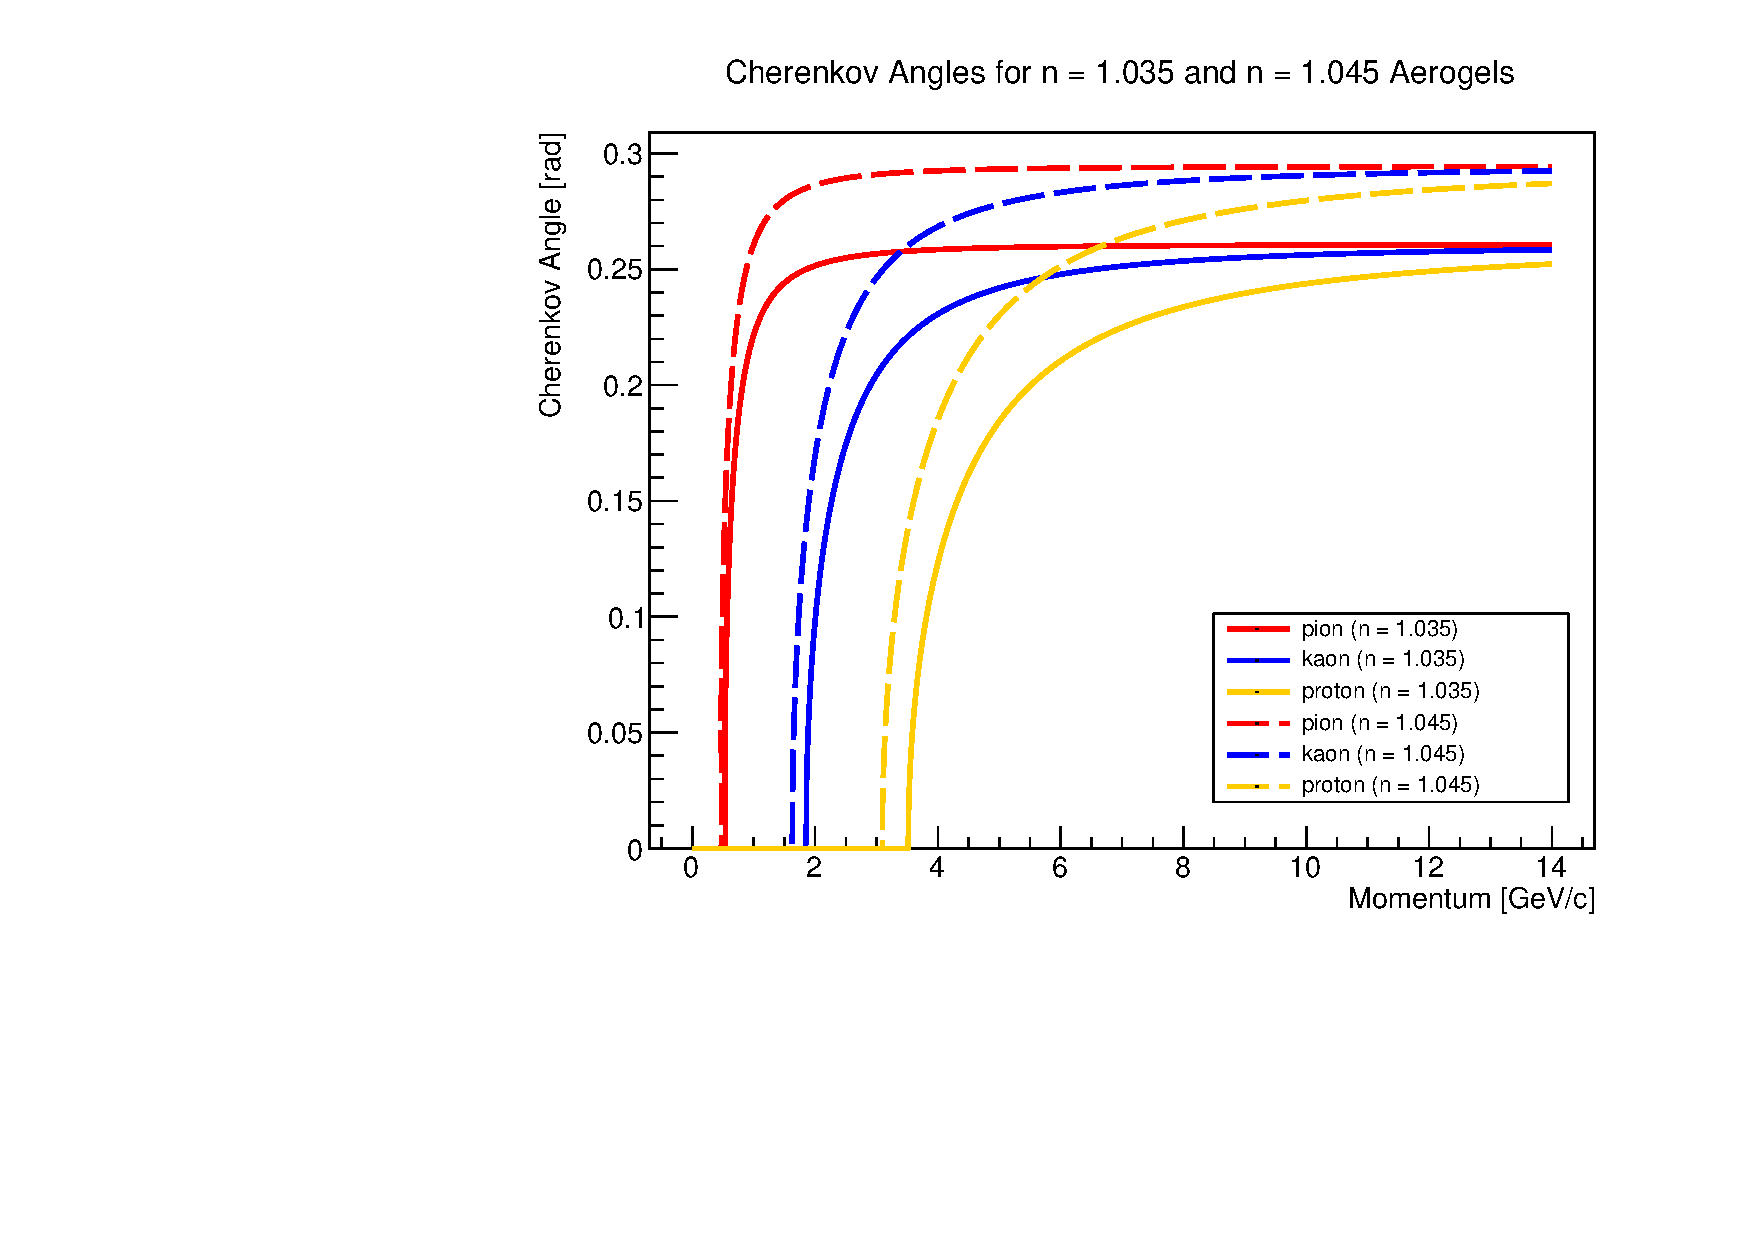
\includegraphics{./figs/changles.pdf}}
\caption[Predicted Cherenkov angles of pions, kaons, and protons over a range of momenta.]{Predicted Cherenkov angles of pions, kaons, and protons over a range of momenta.}
\label{fig:changles}
\end{figure}


A script was written to automate this procedure over a range of different initial particle directions and particle momenta. 
Figure \ref{fig:centeredSeps} shows the separation between likelihood distributions for each particle-particle pair over a range of momenta from 6 GeV/c to 14 GeV/c, with particles travelling directly down the $z$-axis.
The effectiveness of this technique for particle separation can also be measured by looking at misidentification rates: that is, the percentage of the time the particle identity that yielded the minimum negative log-likelihood among the candidate particles was not the true particle.
This is shown in Figure \ref{fig:centeredMis}.

\begin{figure}[]
\centering
\resizebox{0.9\textwidth}{!}{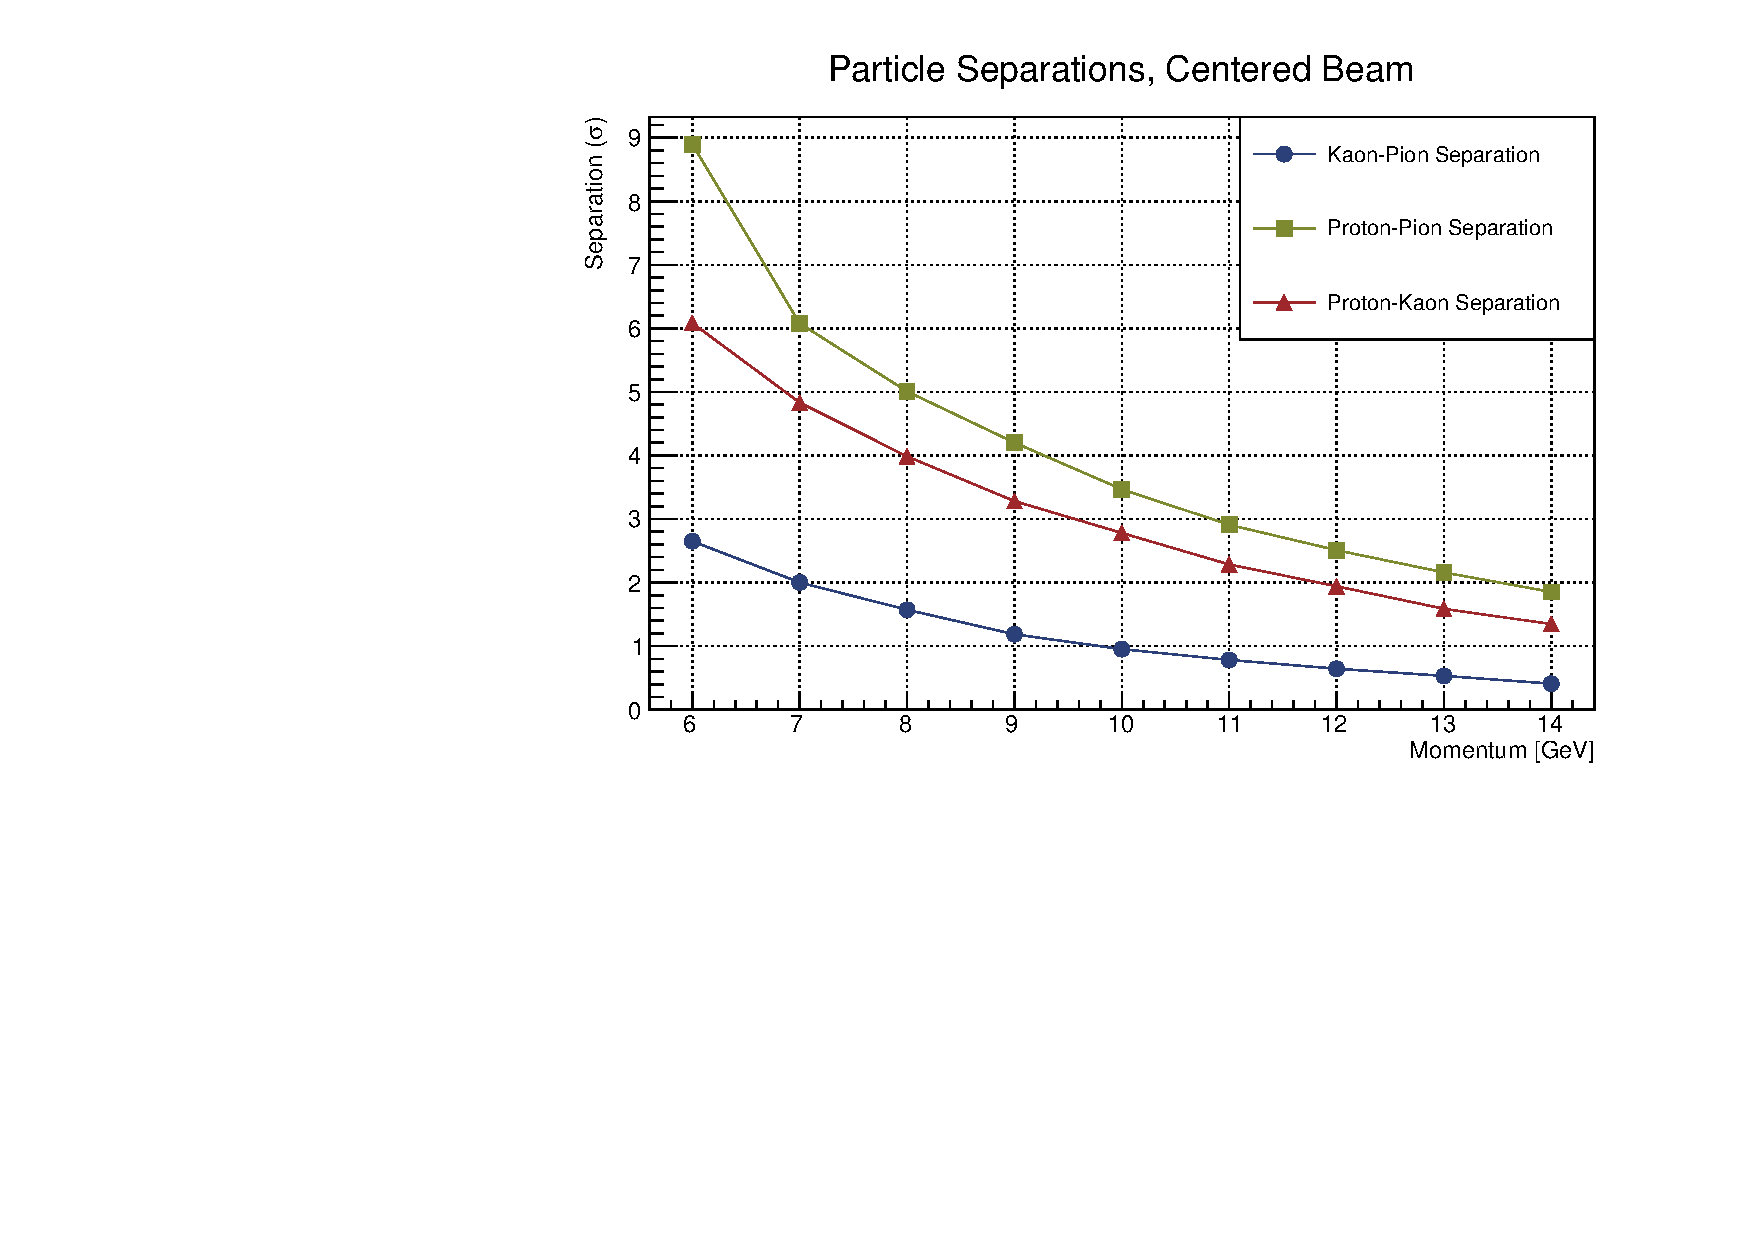
\includegraphics{./figs/centeredSeps.pdf}}
\caption[Plot of the separation between the distributions of computed log-likelihood ratios of different particle pairs, over a range of momenta. ]{Plot of the separation between the distributions of computed log-likelihood ratios of different particle pairs, over a range of momenta. Each ``true" particle was simulated 10,000 times using the Geant4 simulation as entering the aerogel layers with an angle $\theta = 0$ with respect to the downstream axis.}
\label{fig:centeredSeps} 
\end{figure}

\begin{figure}[]
\centering
\resizebox{0.9\textwidth}{!}{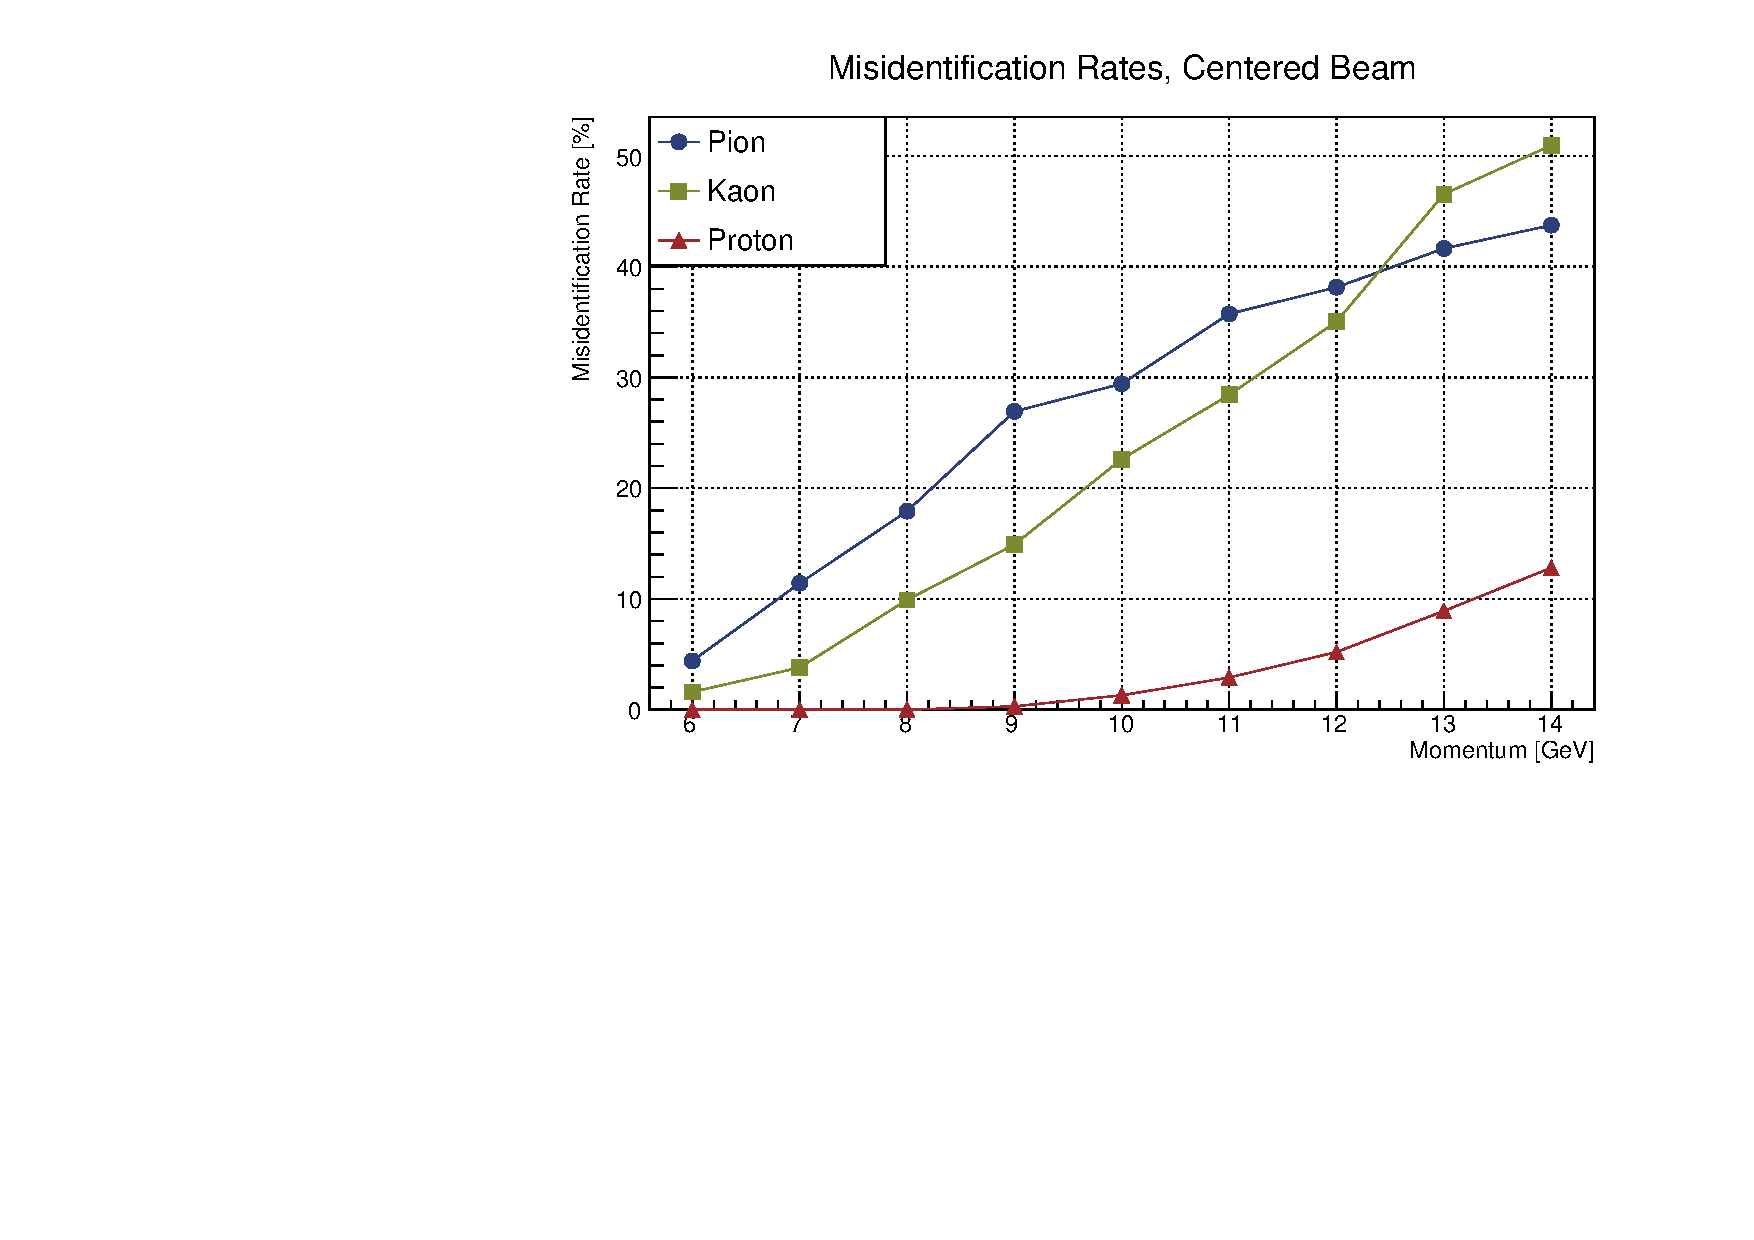
\includegraphics{./figs/centeredMisidentification.pdf}}
\caption[Plot of misidentification rate of the likelihood approach to particle identification over a spectrum of momenta.]{Plot of misidentification rate of the likelihood approach to particle identification over a spectrum of momenta. Each ``true" particle type was simulated 10,000 times using Geant4, and were simulated as entering the aerogel layers with an angle $\theta = 0$ with respect to the downstream axis.}
\label{fig:centeredMis} 
\end{figure}

We see that as momentum increases, we steadily become less effective at distinguishing between pions and kaons - we get a separation greater than $2 \sigma$ past momenta of 7 GeV/c, and at a momentum of 14 GeV/c, we do no better than chance at determining whether a particle is a kaon or pion.
We see that protons remain easily distinguishable from pions and kaons we reach approximately 12 or 13 GeV/c respectively. 

\subsection{Angles}
When particles enter the aerogel at nonzero angles with respect to the beamline axis, a number of intractable effects affect the resulting photon distribution. 
Particles travel further through the aerogel at higher angles and may produce more photons, photons refract differently at higher angles, and the resulting Cherenkov cones may become smeared out over more PMT pixels. 
To evaluate the effectiveness of this likelihood approach across different angles, the procedure described in the preceding section was followed over 5 angular bins ranging from 0 to 0.4 radians.
The resulting particle separations are shown in Figure \ref{fig:angleSeps}.

It is clear that as the angle of the incident particle increases, we become better able to separate out our particles from one another up until a certain point.
This is likely because the photon rings are ``smeared out" over several different PMT pixels, allowing for finer details to be measured. 
However, past 0.35 radians we see that our ability to distinguish particles significantly decreases.
This is because at this point, the photon rings partially fall off of the detector plane, and with fewer detected photons, there is less information to distinguish particles.

\begin{figure}[]
\centering
\resizebox{0.9\textwidth}{!}{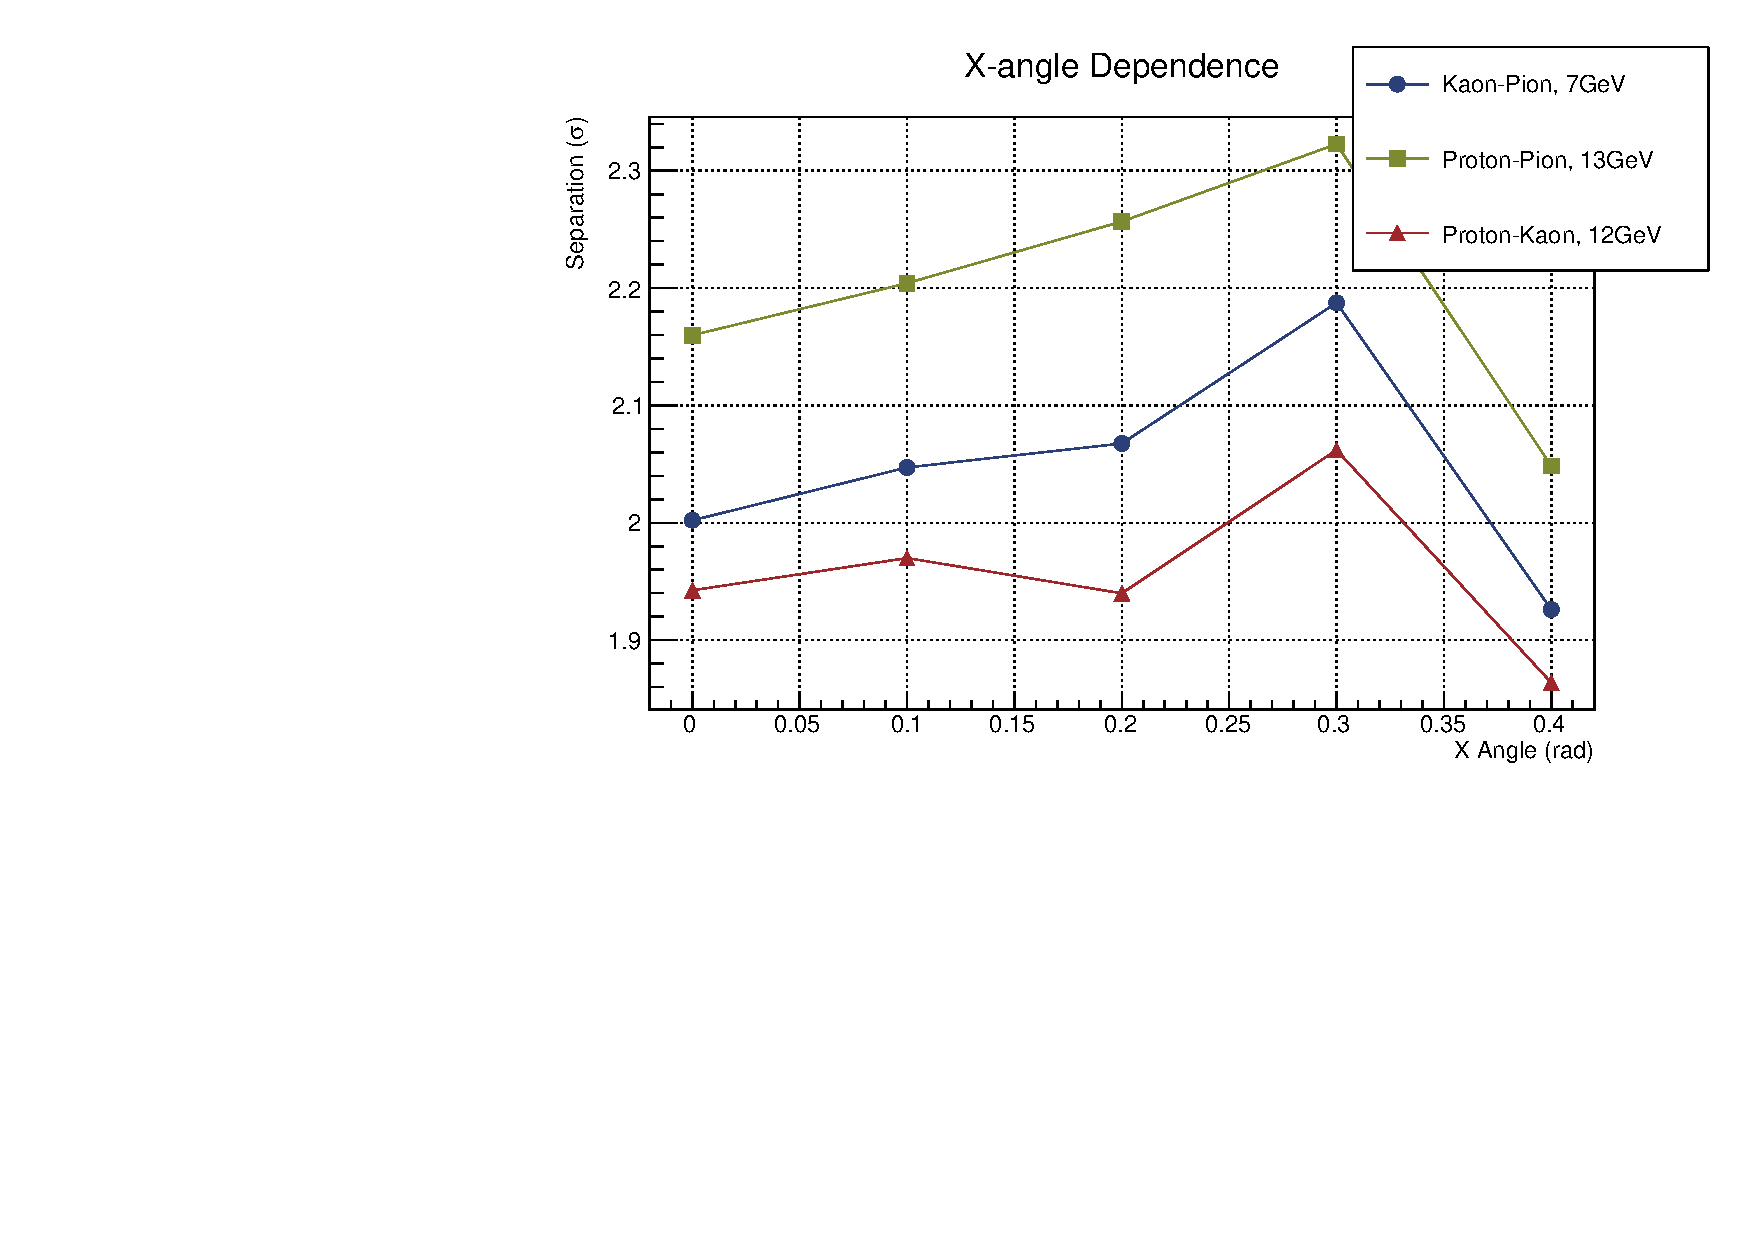
\includegraphics{./figs/xAngleSeps.pdf}}
\caption[Plot of the separation between the distributions of computed log-likelihood ratios of different particle pairs, over a range of angles. ]{Plot of the separation between the distributions of computed log-likelihood ratios of different particle pairs, over a range of angles. Each particle is simulated 10,000 times using the Geant4 simulation as entering the aerogel layers with an angle with respect to the downstream axis. \TODO{reword this}}\label{fig:angleSeps}
\end{figure}


\section{Multi-particle events}
\label{sec:multiparticle}
Although so far only single-photon ring events have been evaluated, it is often the case that the photons from several different particles will be detected at the same time in the ARICH detector. 
It is necessary that the likelihood particle identification technique is able to separate out multi-particle events as well. 

To accomplish this, the simulation was modified to take in an array of different particle momenta, positions, and directions, rather than just one set of parameters.
Because the photon rings from each particle may overlap with one another and cannot necessarily be disentangled, every possible combination of particle hypotheses must be simulated and compared to the event data in order to concurrently fit all particles.
Because the photon probability distribution functions for each particle are independent, each particle is independently simulated for each particle hypothesis, and the resulting photon histograms are saved.
Next, for every possible combination of these particle hypotheses, we sum together the corresponding particles' photon distribution histograms and calculate a log-likelihood by comparing the sum to the event data.
In total, for $n$ detected particles and $p$ possible particle hypotheses, we must simulate $p \times n$ photon distribution functions, do $p^n$  log-likelihood comparisons with our event data, and select the combination with the minimum negative log-likelihood from these $p^n$ options. 

An example of the result of this process demonstrated in Figure \ref{fig:multiParticle}. A three-particle event was simulated, consisting of one kaon, one pion, and one proton. 
Each particle had a momentum randomly drawn from a Gaussian with a mean of $10$ GeV/c and a standard deviation of $2$ GeV/c, with directions thrown from a Gaussian with a mean of $0$ rad and standard deviation of $0.3$ rad, and with initial positions drawn from a Gaussian with a mean of $0$ and a standard deviation of $2$ cm.
The values for their momenta, positions, and directions were then used as inputs to the fast simulation, and the likelihoods of each of the 27 possible particle combinations were calculated.
In this particular example, the particle identification code was able correctly the identify the ``true" combination of particle types.
However, this was an arbitrary test - real experimental data would not necessarily resemble distributions such as this.

\begin{figure}[]
\centering
\resizebox{0.9\textwidth}{!}{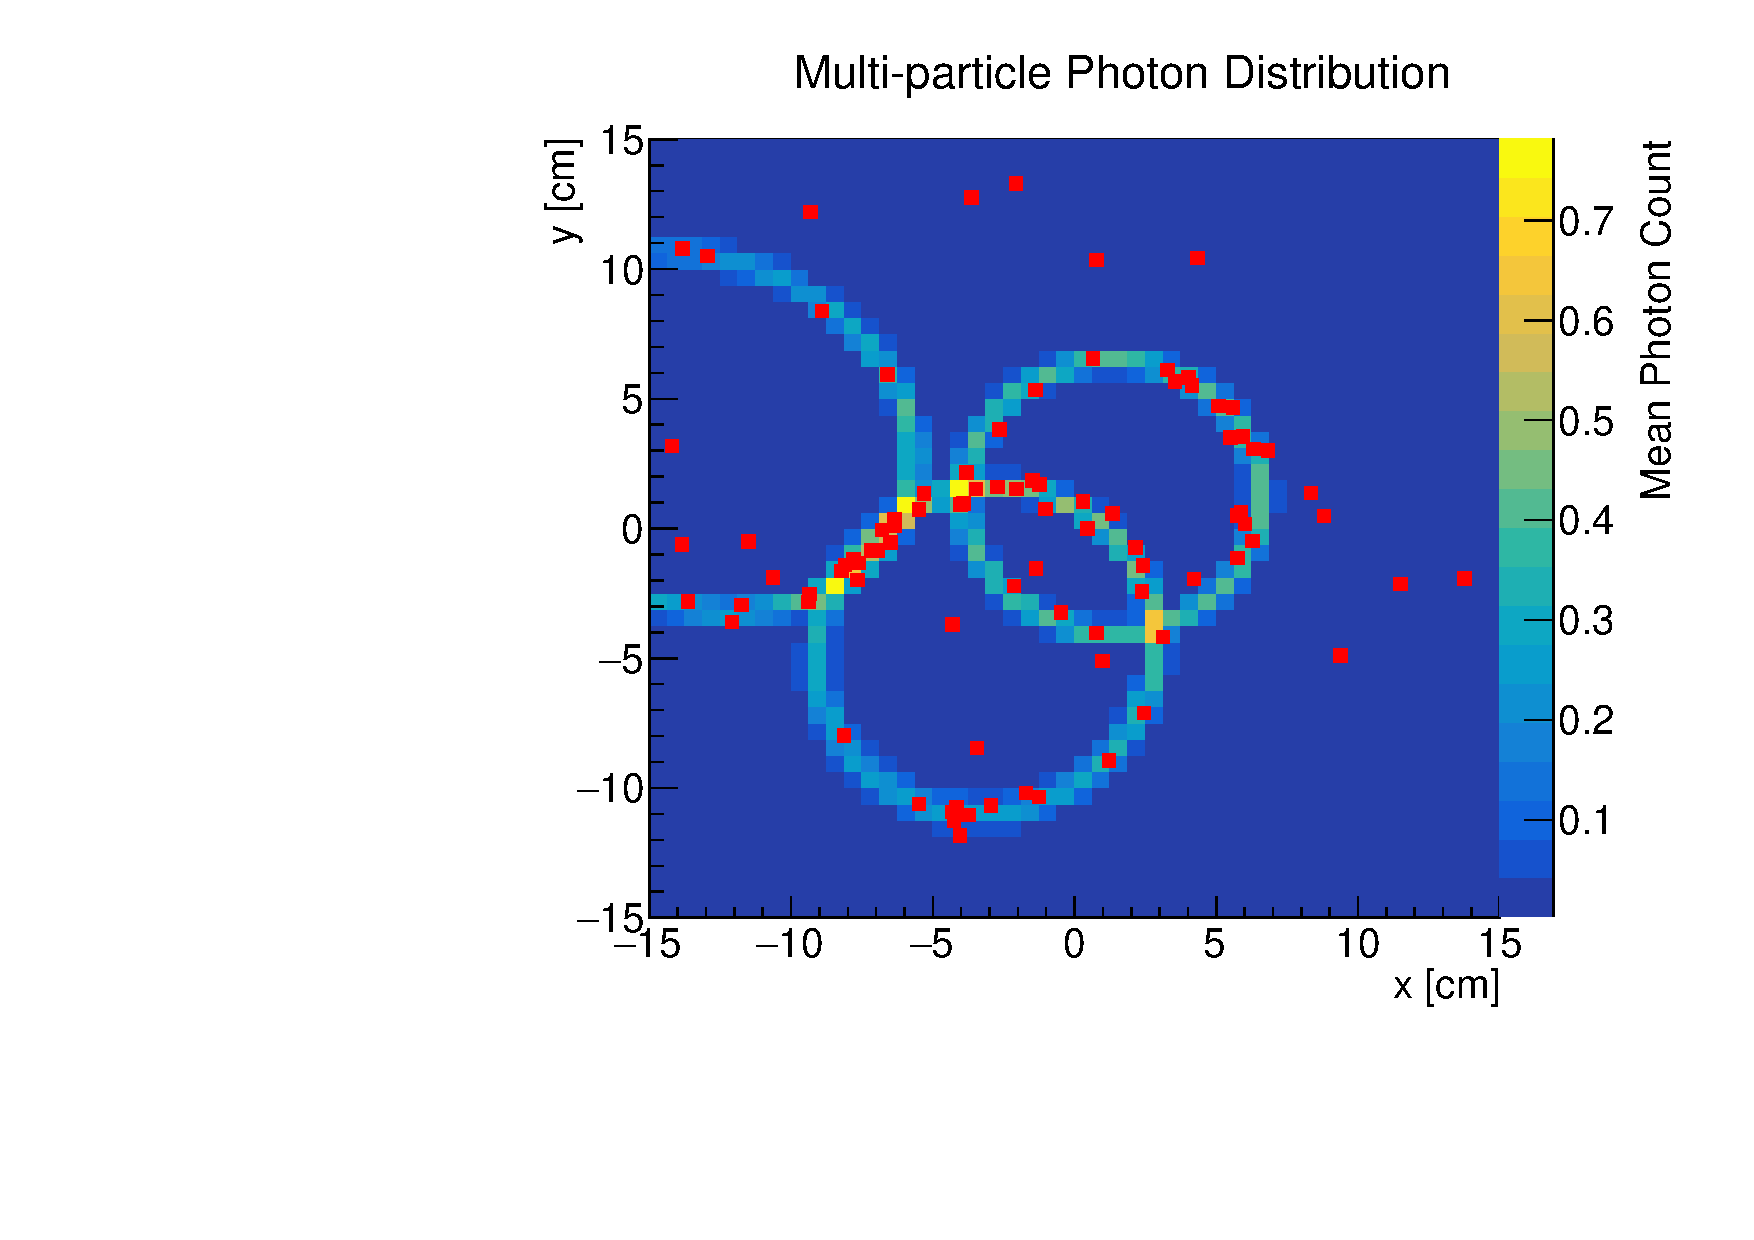
\includegraphics{./figs/pdfMultiParticle.pdf}}
\caption[Simulated event data and expected photon distribution for a three-particle event]{Histogram of photons detected in a simulated event (shown in red) overlaid on the photon distribution of the best-fit particle hypothesis for the data, corresponding to a pion, a kaon, and a proton.}
\label{fig:multiParticle} 
\end{figure}


\endinput

Any text after an \endinput is ignored.
You could put scraps here or things in progress.
